\documentclass[final, 9pt, twocolumn]{saucis}
\usepackage{cite}
\usepackage{float}
\usepackage{epsfig}
\usepackage{epstopdf}
\usepackage{orcidlink}
\usepackage{rorlink}
\usepackage{url}
\let\CheckCommand\providecommand
\usepackage{microtype}
\usepackage{lmodern}
\usepackage{textcomp}
\usepackage{afterpage}

\newcommand{\y}{2026} %year\renewcommand{\saucisAuthors}{Student Name} %author names

\renewcommand{\saucisJD}{RESEARCH ARTICLE}
\startsAtpage{0} %page number start point

\begin{document}

%---------------------------------------------------------------------------------
%	TITLE
%---------------------------------------------------------------------------------

\title{Aging domain names: When Do Attackers Weaponize Newly Registered Domains? }

%---------------------------------------------------------------------------------
%	AUTHORS
%---------------------------------------------------------------------------------
\author[1*]{Adam Khalid, Elza Latifi, Felix Picon}

\affil[1]{Cybersecurity, Operating Sytstem and Networking Master}
\date{\today}
%---------------------------------------------------------------------------------
%	ABSTRACT
%---------------------------------------------------------------------------------

\saucisAbstract{
This study investigates the lifecycle of malicious domain names, focusing on the delay between their registration and their deployment for malicious activities ("aging"). Using a dataset of 653,989 domains that underwent a WHOIS-based takedown, we analyze three key hypotheses regarding their aging, attack patterns, and takedown responsiveness. Our results show that attackers predominantly use a "hit-and-run" strategy: the median aging time is only 4.2 days, indicating that domains are weaponized almost immediately after creation. We also identify strong attack patterns, with unspecified targets ("Other") representing 26.1\% and the United States Postal Service (USPS) being the primary identifiable target for 9.1\% of the analyzed domains, and the .com TLD accounting for 23.2\% of registrations, followed closely by .top (19.6\%). Critically, we identify that technical or administrative WHOIS updates consistently act as a precursor to weaponization, functioning as a "wake-up signal" roughly 72 hours before an attack. Finally, we measure the effectiveness of countermeasures, observing a median takedown time of 35.8 hours (approx. 1.5 days), with WHOIS-specific takedowns being significantly faster (median 11.9 hours). These findings suggest that defense mechanisms must prioritize real-time detection over reputation-based aging metrics for this category of threats.
}
%---------------------------------------------------------------------------------
%	KEYWORDS 
%---------------------------------------------------------------------------------
\saucisKeywords{Malicious Domains, Phishing, Domain Aging, Takedown Analysis, WHOIS, Cybersecurity}
%---------------------------------------------------------------------------------
%	ARTICLE INFO
%---------------------------------------------------------------------------------
\saucisonline{13 February 2026}
\maketitle

\section{Introduction}

The Domain Name System (DNS) is a critical infrastructure, yet it remains fundamentally vulnerable to abuse by cybercriminals who rely on it to host phishing pages, command and control (C2) servers, and malware distribution networks \cite{dns_abuse_framework}. Historically, a common defensive heuristic to detect such infrastructure has been "domain aging": the premise that newly registered domains (NRDs) are inherently more suspicious, whereas older domains are more likely to be legitimate. 

However, recent research indicates that relying solely on domain age is an insufficient and easily manipulated metric. Systems distinguishing between domains registered specifically for malicious purposes and benign domains that were later compromised reveal stark behavioral differences: while compromised domains are typically older, the vast majority of maliciously registered domains are weaponized almost immediately, with a significant portion being blacklisted on the very day of their registration \cite{comar_aging}. Furthermore, sophisticated attackers increasingly employ "domain aging" tactics—registering domains and leaving them dormant for months to bypass reputation-based filters before deploying their attacks \cite{comar_evasion}. 

This paper addresses a critical gap in the understanding of attacker operational security: \textit{Under what specific timelines and structural patterns do attackers weaponize newly registered domains?} We focus exclusively on a dataset of domains that underwent WHOIS-based takedowns (e.g., due to fraudulent registration data). This subset is particularly relevant as it represents a distinct category of DNS abuse where the registration process itself is illicit, providing a clear contractual basis for rapid mitigation by registrars and registries.

Through the empirical analysis of this dataset, we evaluate three core hypotheses:
\begin{itemize}
    \item \textbf{H1 (Aging and Weaponization):} Rather than systematically employing "domain aging" techniques to bypass security filters, attackers predominantly favor a rapid "hit-and-run" strategy for maliciously registered domains.
    \item \textbf{H2 (Structural Patterns):} Attack infrastructures are not uniformly distributed but are disproportionately concentrated in specific Top-Level Domains (TLDs)—driven by low-cost economic models—and targeted toward high-interaction sectors such as logistics.
    \item \textbf{H3 (Mitigation Resilience):} The operational responsiveness (time to takedown) varies significantly depending on the mitigation vector, with WHOIS compliance mechanisms yielding systematically faster disruption than content-based abuse reporting.
\end{itemize}

By validating these hypotheses, this study aims to refine real-time detection mechanisms and provide actionable intelligence for registrars and cybersecurity practitioners to prioritize mitigation efforts against fraudulent registrations.

\section{Background and Related Work}

To effectively analyze the lifecycle and weaponization of malicious domains, it is imperative to establish a clear taxonomy of Domain Name System (DNS) abuse and understand the traditional heuristics used by the cybersecurity industry.

\subsection{Maliciously Registered vs. Compromised Domains}
A fundamental prerequisite in DNS abuse research is the operational distinction between two fundamentally different types of abusive infrastructure: maliciously registered domains and compromised domains \cite{comar_classification}. 

Maliciously Registered Domains are created by cybercriminals with the explicit and sole intention of conducting fraudulent activities, such as phishing campaigns, malware distribution, or botnet command and control \cite{comar_classification, apwg_trends}. These domains exhibit distinct structural characteristics. For instance, they tend to be technically minimalist: nearly 71.8\% of them do not deploy any specific web technologies on their homepage, as they are often designed to serve phishing pages directly via subdomains, specific URL paths, or simple HTTP redirections \cite{comar_technologies}. Furthermore, attackers frequently incorporate highly deceptive keywords (e.g., "online," "bank," "secure," "support") directly into the domain name strings to trick victims into divulging their credentials \cite{comar_lexical_phishing}.

In contrast, Compromised Domains are initially registered by benign users for legitimate purposes but are subsequently hijacked by attackers \cite{comar_classification}. This exploitation typically occurs at the hosting level rather than the DNS level, often due to vulnerabilities in outdated web applications or Content Management Systems (CMS) like WordPress \cite{comar_classification, comar_aging}. Consequently, compromised domains are technically much more complex; approximately 67.7\% of them utilize more than six different web frameworks and plugins, reflecting the effort of legitimate owners to build fully functional websites \cite{comar_technologies}. From a mitigation perspective, while maliciously registered domains can be safely blocked at the DNS level (e.g., removed from the zone file by registrars), compromised domains require targeted content takedowns at the hosting level to avoid collateral damage to legitimate services \cite{dns_abuse_framework, comar_mitigation}.

\subsection{The "Domain Aging" Heuristic and Evasion Mechanisms}
Historically, "domain age"—defined as the time elapsed between a domain's registration and its deployment or detection—has been a cornerstone heuristic for security monitoring bodies to evaluate the reputation of an infrastructure \cite{comar_classification, comar_evasion}. The underlying assumption is that older domains are inherently more trustworthy \cite{comar_aging}. 

Empirical data partially supports this bias for compromised domains: approximately 57\% of compromised domains were registered at least six years before being blacklisted \cite{comar_aging}. This correlation is logical, as older websites are more likely to run deprecated, vulnerable software stacks \cite{comar_aging}. Conversely, maliciously registered domains generally exhibit an extremely short, "hit-and-run" lifecycle. For 84\% of these domains, the delay between registration and blacklisting is less than a year, and 13\% are weaponized and blacklisted on the exact same day they are registered \cite{comar_aging}. 

However, relying strictly on age-based metrics has become increasingly problematic due to sophisticated evasion mechanisms developed by cybercriminals \cite{comar_evasion}. Aware of reputation filters, sophisticated attackers actively employ a tactic known as "domain aging" \cite{comar_evasion}. This technique involves registering domain names and deliberately leaving them dormant for weeks or even months before utilizing them in phishing attacks \cite{comar_evasion}. The strategic goal is to artificially mature the domain's reputation, thereby bypassing security controls that automatically flag or block newly registered domains \cite{comar_evasion}. 

Because of these evasion tactics, age alone is an insufficient discriminant \cite{comar_evasion}. Automated classification systems evaluating domain reputation demonstrate that age must be contextualized alongside multiple other features—such as lexical analysis, the number of web technologies, and the use of TLS certificates—to accurately distinguish a deliberately aged malicious domain from a genuinely old but recently compromised legitimate site \cite{comar_classification, comar_aging}.


\section{Methodology}

\subsection{Dataset}
The initial dataset of malicious domains and their corresponding uptime monitoring logs, collected between 2022 and 2025, was provided by Yevheniya Nosyk. From this corpus, we isolated domains that experienced a takedown event specifically linked to WHOIS policy violations (e.g., fraudulent or inaccurate registration data). This filtering. This resulted in a comprehensive analytical dataset of 653,989 domains.

\subsection{Takedown Identification}
To systematically distinguish WHOIS-based takedowns from other mechanisms (such as content-based or DNS blocklist takedowns), we programmatically parsed the uptime records of each domain. A takedown was strictly classified as WHOIS-linked if the dataset's metadata flagged the primary takedown reason as "whois", or if the distinct list of recorded takedown actions for that domain explicitly included a "whois" event type. This automated filtering ensured that our analysis uniquely focuses on infrastructural takedowns mediated by registrars or registries.

\subsection{Data Limitations and Potential Biases}
While the dataset is extensive, it is important to acknowledge potential biases. The monitoring system may inherently over-represent certain top-level domains (TLDs) or regions based on the geographic distribution of its sensing infrastructure and the specific threat feeds utilized. Additionally, for the year 2022, our dataset only contains detections for the month of December; thus, longitudinal comparisons involving 2022 data are treated with caution.


\subsection{Metrics}
For each domain, we calculated two primary, time-based metrics:
\begin{enumerate}
    \item \textbf{Aging (Days):} The time interval between the domain's creation date (from WHOIS records) and its first reported discovery as malicious.
    \item \textbf{Takedown Delay (Hours):} The time interval between the discovery of the domain and its effective takedown (transition to NXDOMAIN or hold status).
\end{enumerate}

To reconstruct the life cycle of the identified threats, we used key temporal metrics:

\begin{itemize}
    \item \textbf{Aging Time}: Calculated as $T_{discovery} - T_{creation}$, measuring the interval between the domain's registration and its first reported malicious activity.
    \item \textbf{WHOIS Update Delay}: Computed as $T_{discovery} - T_{update}$, identifying the delay between the last administrative or technical modification in WHOIS and the attack.
    \item \textbf{Remaining Validity}: Calculated as $T_{expiration} - T_{discovery}$, representing the contractual time remaining before the domain's expiration at the moment of detection.
    \item \textbf{Operational Survival}: Extracted from raw monitoring data, this represents the duration in hours between the initial discovery and the effective suspension (e.g., NXDOMAIN status).
\end{itemize}

\subsection{Statistical Testing}
To rigorously assess the disparity in aging strategies between high-volume and high-precision TLDs, we conducted a Mann–Whitney U test comparing the aging time distributions of \textit{.top} and \textit{.com} domains. This non-parametric test evaluates whether the two groups exhibit genuinely different behaviors or whether the observed differences could be attributed to random variation. Unlike simple comparisons of means, it considers the full distribution of values, making it more robust to skewed data and outliers.

The test reveals a highly significant difference ($p < 0.001$), with median aging times of 2.6 days for \textit{.top} domains and 7.9 days for \textit{.com} domains.

This result provides strong statistical evidence that weaponization timelines differ substantially across TLDs, supporting the hypothesis that attackers adapt their strategies based on infrastructure cost and domain reputation.

Let $n_1$ and $n_2$ denote the number of \textit{.top} and \textit{.com} domains, respectively, and $R_1$ the sum of ranks for the \textit{.top} group. The Mann–Whitney U statistic is computed as:

\begin{equation}
U_{\textit{.top}} = n_1 n_2 + \frac{n_1(n_1+1)}{2} - R_1
\end{equation}

For example, if $n_1 = X$, $n_2 = Y$, and $R_1 = Z$, then:

\begin{equation}
U_{\textit{.top}} = X \cdot Y + \frac{X(X+1)}{2} - Z
\end{equation}

Similarly, the statistic for the second group is:

\begin{equation}
U_{\textit{.com}} = n_1 n_2 - U_{\textit{.top}}
\end{equation}

In practice, the smaller of $U_{\textit{.top}}$ and $U_{\textit{.com}}$ is used to compute the two-sided $p$-value.
\section{Baseline Statistical Results}

\subsection{Hypothesis 1: Domain Aging}
Contrary to the hypothesis that attackers "age" their domains, our primary analysis reveals a strategy of relatively immediate utilization, though with a persistent long-tail.
    \begin{itemize}
        \item \textbf{Median Aging:} 4.2 days
        \item \textbf{Mean Aging:} 112.3 days
    \end{itemize}
The low median indicates that the majority of domains are weaponized within a few days of registration (with 54\% of domains used in $\le$5 days). The higher mean suggests a long tail of outliers, but the dominant behavior is "hit-and-run".

\begin{figure}[htbp]
		\centering
			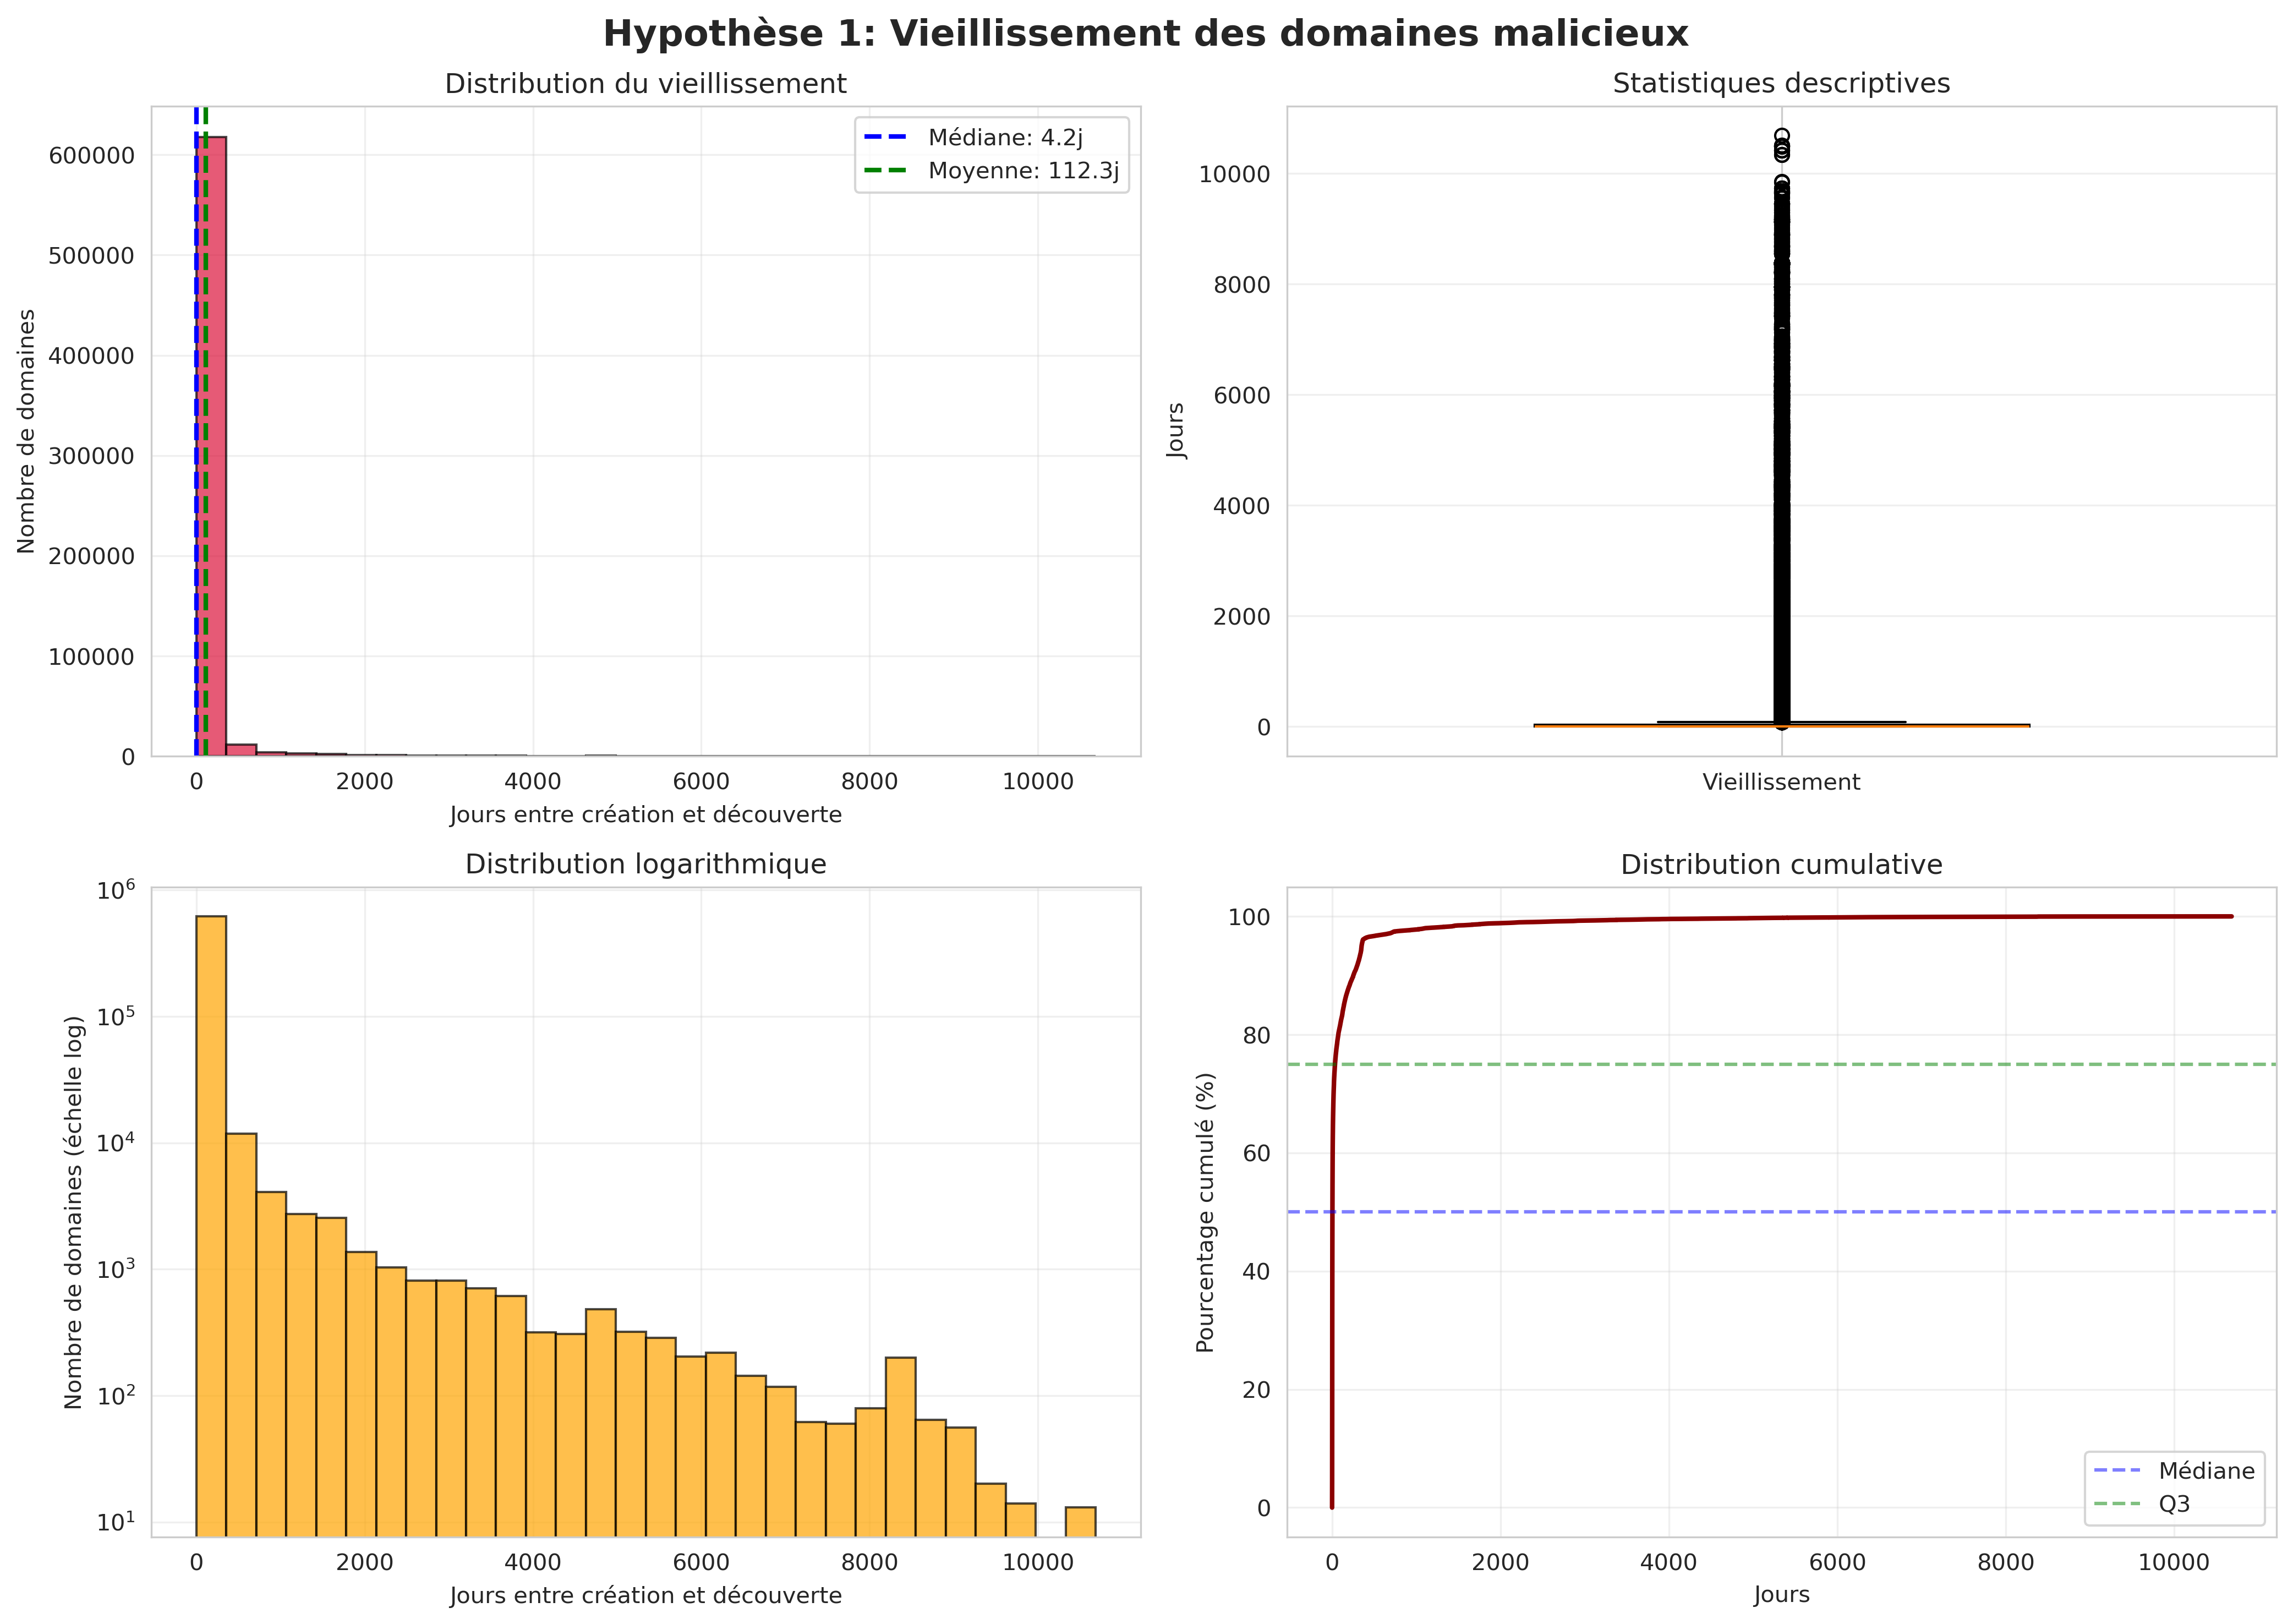
\includegraphics[width=0.45\textwidth]{analysis_results/graphs_sample/hypothesis1_aging_full.png} 
	\caption{Distribution of domain aging (days between creation and discovery).}
	\label{fig:aging}
\end{figure}

\subsection{Hypothesis 2: Attack Patterns}
The data reveals highly concentrated attack vectors associated with specific brands and top-level domains (TLDs).

\textbf{Top Targets:}
The dataset is diverse, but heavily impacted by "Other" uncategorized targets and logistics services.
\begin{itemize}
    \item \textbf{Other:} 170,649 domains (26.1\%)
    \item \textbf{USPS:} 59,463 domains (9.1\%)
    \item \textbf{Generic/Spear Phishing:} 41,336 domains (6.3\%)
\end{itemize}

\begin{figure}[htbp]
		\centering
			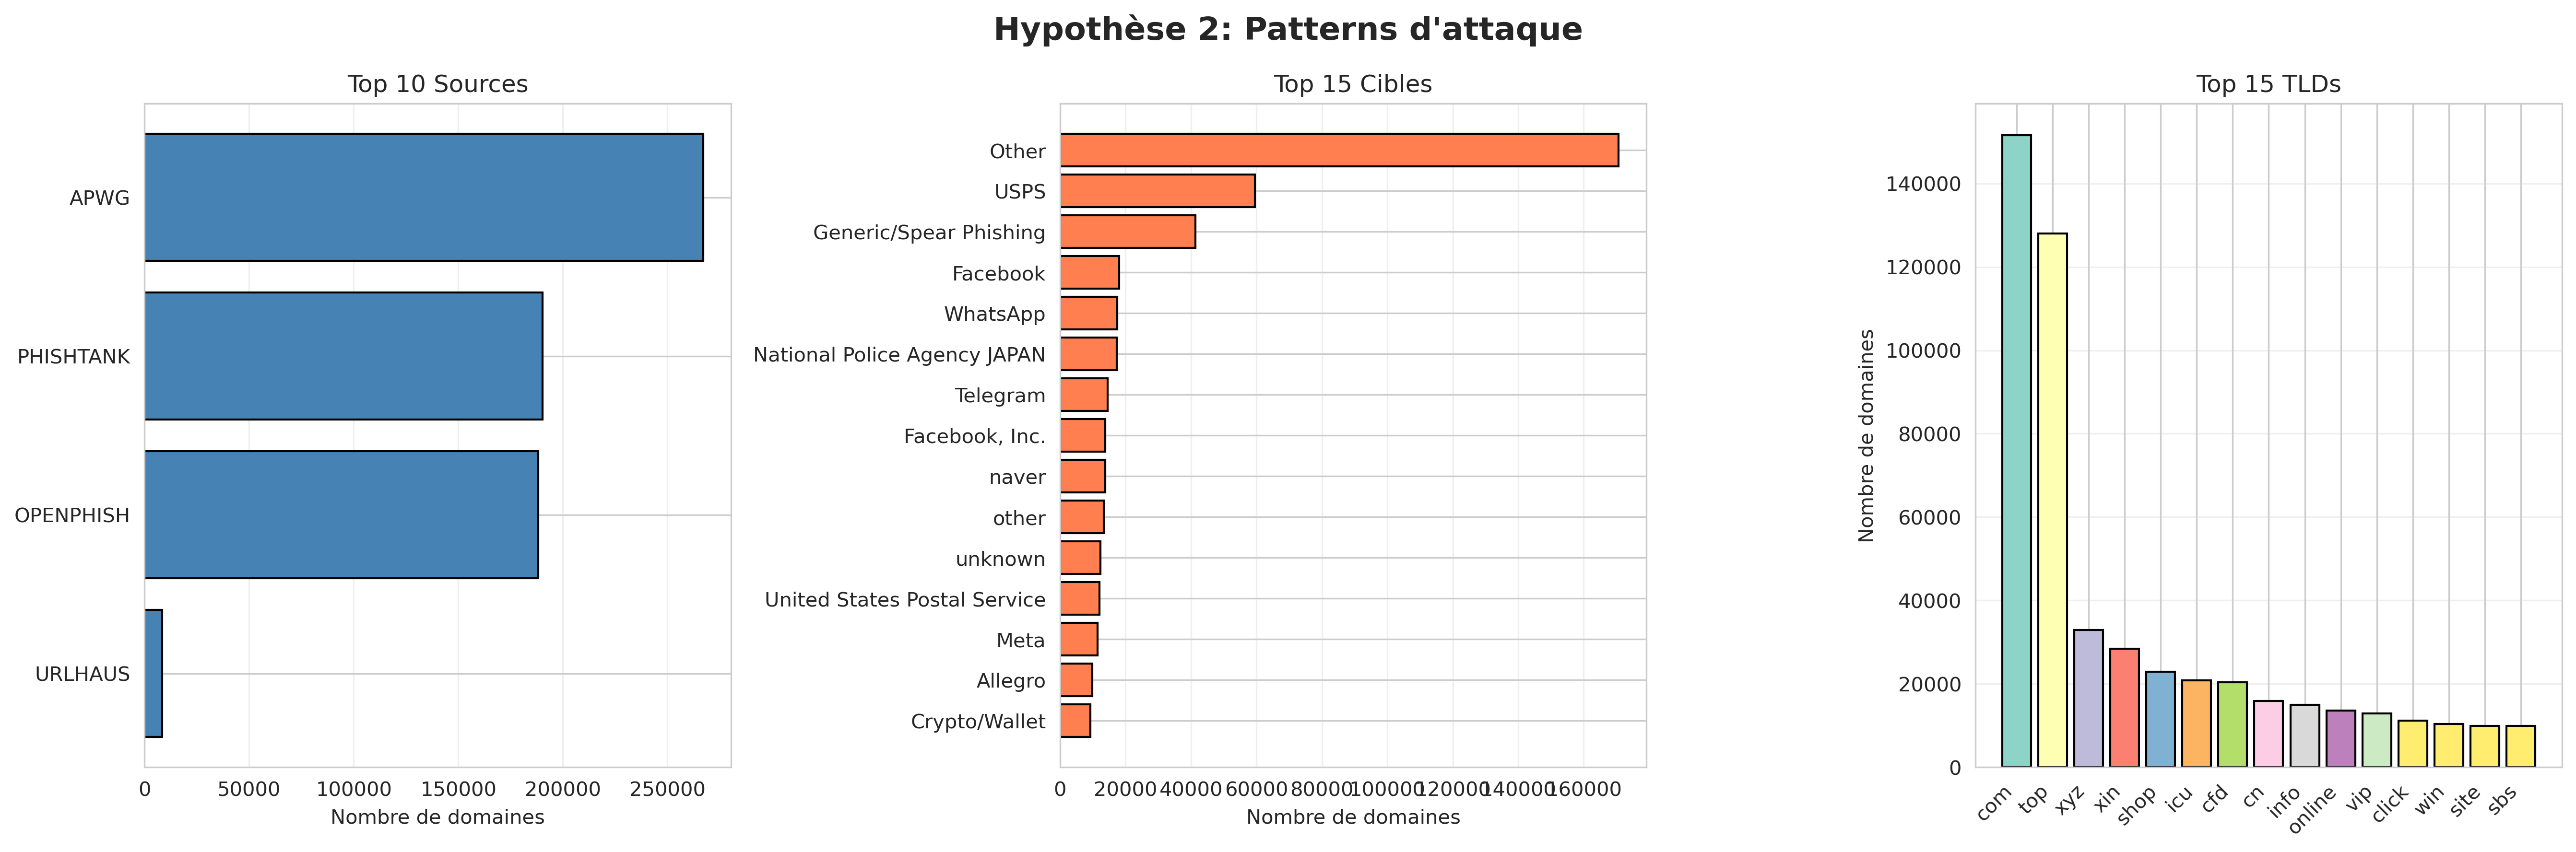
\includegraphics[width=0.45\textwidth]{analysis_results/graphs_sample/hypothesis2_patterns_full.png} 
	\caption{Top sources, targets, and TLDs observed in the dataset.}
	\label{fig:patterns}
\end{figure}

\textbf{Top TLDs:}
Common and permissive TLDs are predominantly preferred by attackers in this dataset.
\begin{itemize}
    \item \textbf{.com:} 151,564 domains (23.2\%)
    \item \textbf{.top:} 128,001 domains (19.6\%)
    \item \textbf{.xyz:} 32,924 domains (5.0\%)
\end{itemize}


\subsection{Hypothesis 3: Takedown Efficiency}

\begin{figure}[htbp]
		\centering
			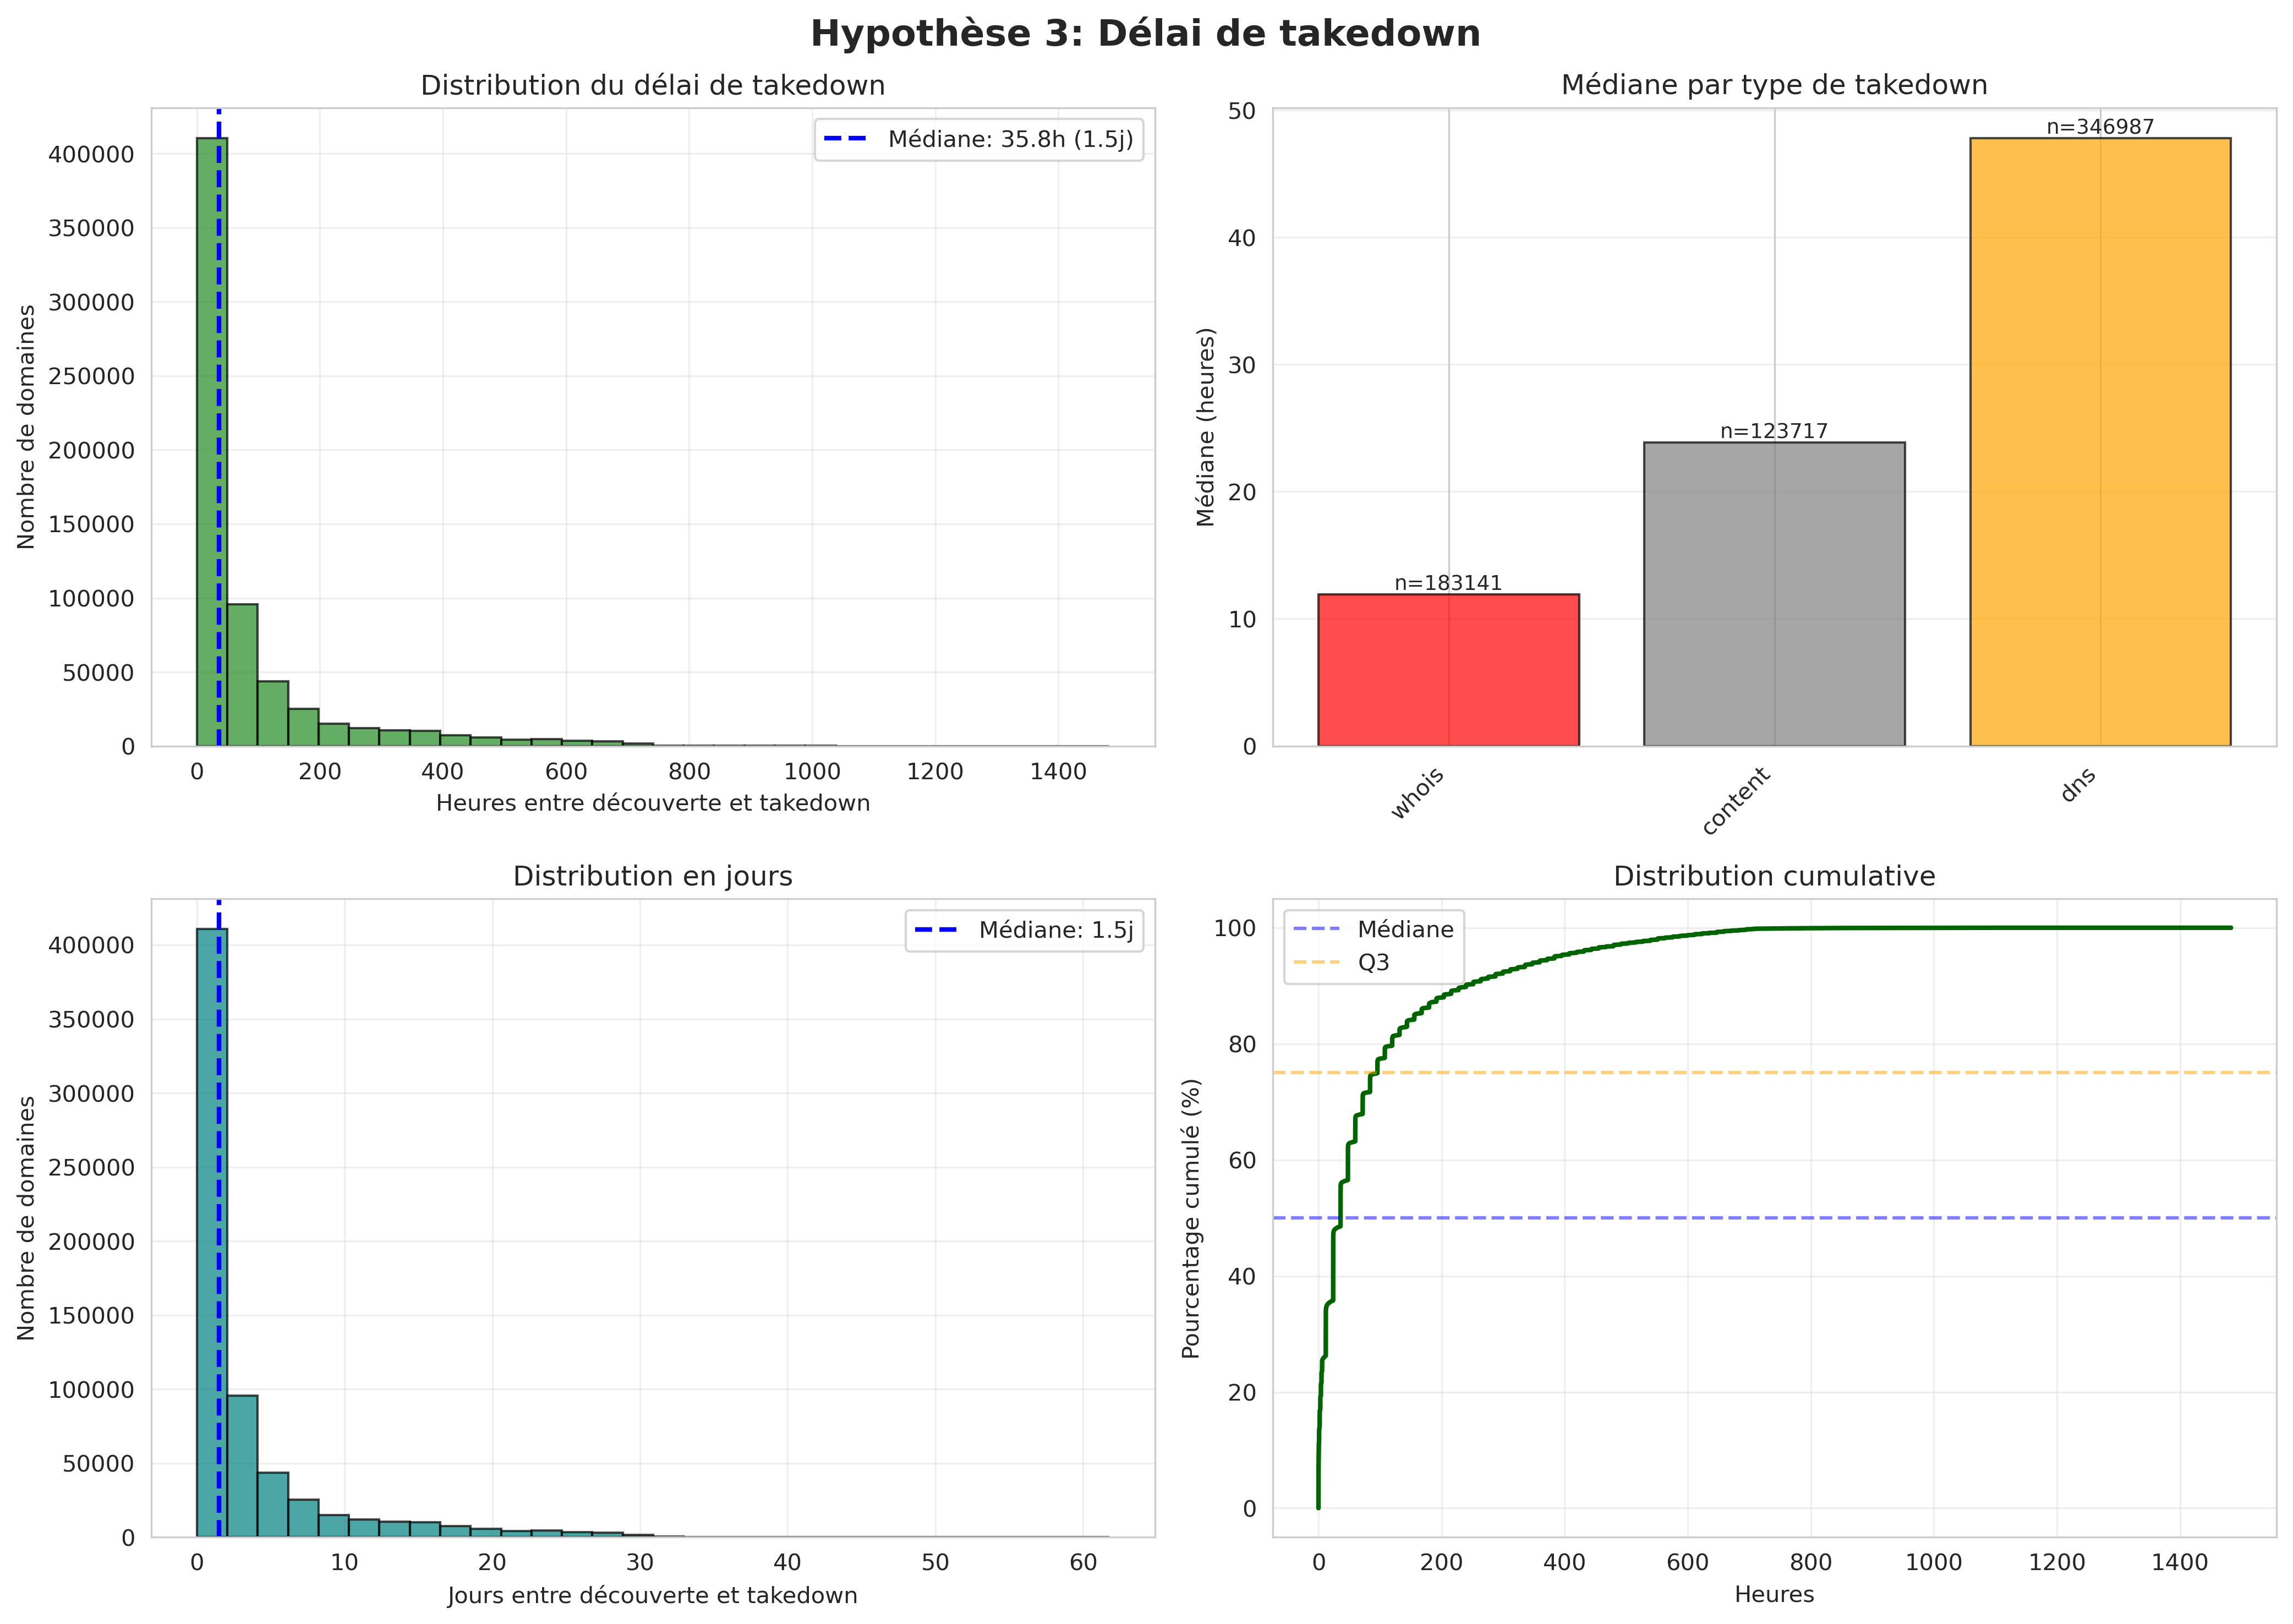
\includegraphics[width=0.45\textwidth]{analysis_results/graphs_sample/hypothesis3_takedown_full.png} 
	\caption{Distribution of takedown delays.}
	\label{fig:takedown}
\end{figure}


% Transition into socio-economic analysis
The preceding sections established the core temporal patterns and defensive response times for maliciously registered domains. To understand why certain domains are weaponized immediately while others are incubated, it is essential to examine the 
technical and economic choices available to attackers (e.g., TLD selection, registrar behavior, and domain naming strategy).

\section{The Socio-Economic Ecosystem}

Analysis shows that the choice of technical resources (TLD, Registrar, Domain name length ) is closely linked to the attack's objective.

\subsection{Correlation between TLD cost and aging strategy}
The graph (Figure \ref{fig:strategic_ratio_tld}) reveals a clear divide between "Low-cost" extensions and established extensions.

\begin{figure}[htbp]
    \centering
    
\includegraphics[width=\linewidth]{analysis_results/graphs_jpg/strategic_ratio_tld.jpg}
    \caption{Strategic distribution (Incubation vs. Direct Weaponization) across top TLDs.}
    \label{fig:strategic_ratio_tld}
\end{figure}

\begin{itemize}
    \item \textbf{Volume strategy:} Extensions like .xin, .icu, or .top, characterized by their low acquisition cost, are used over 80\% of the time for Direct Weaponization. For the attacker, these domains are disposable consumables. This pattern strongly suggests a \textbf{volume-based opportunistic approach}, typical of mass spam or wide-scale phishing campaigns.
    \item \textbf{Precision strategy:} Conversely, .com and especially .cn show much higher incubation rates. The higher cost and stricter administrative controls of these extensions push attackers to protect their investment by letting the domain age to ensure it passes security filters. This behavior is indicative of a high-precision targeted phishing approach, where domain credibility is prioritized to deceive more vigilant victims and bypass advanced organizational defenses. 
\end{itemize}

To statistically validate this disparity in aging strategies between high-volume and high-precision TLDs, we performed a Mann-Whitney U test comparing the aging distributions of domains under the \textit{.top} and \textit{.com} extensions. The test yielded a highly significant p-value ($p < 0.001$), with median aging times of 2.6 days for \textit{.top} domains and 7.9 days for \textit{.com} domains. This confirms a statistically significant difference in their weaponization timelines, strongly supporting the hypothesis that attackers employ distinct strategies based on infrastructure cost and reputation.


\subsection{Registrar Specialization}
This logic is confirmed at the registrar level (Figure \ref{fig:strategic_ratio_registrars}).

\begin{figure}[htbp]
    \centering
    
\includegraphics[width=\linewidth]{analysis_results/graphs_jpg/strategic_ratio_registrars.jpg}
    \caption{Strategic specialization of the top 10 Registrars.}
    \label{fig:strategic_ratio_registrars}
\end{figure}

We observe that entities like Dominet or Nicenic (based in Asia) act as factories for "Direct Weaponization." They offer maximum reactivity for short-lived campaigns. In contrast, players like NameCheap or Gname host a much larger proportion of "aging" domain names (over 40\% incubation). These platforms are chosen for their stability, allowing the domain to remain dormant without being suspended prematurely.

\subsection{Target Influence and Lexical Credibility}
The ecosystem analysis concludes with the study of the targets' nature and the structure of the domain names.\\

The data shows that the aging strategy is closely linked to the target's reputation (Figure \ref{fig:aging_by_brand}).

\begin{figure}[htbp]
    \centering
    
\includegraphics[width=\linewidth]{analysis_results/graphs_jpg/aging_by_brand.jpg}
    \caption{Median and P90 aging time according to the targeted brand.}
    \label{fig:aging_by_brand}
\end{figure}

\begin{itemize}
    \item For entities requiring absolute trust, such as the Japanese Police or Naver (South Korea's leading web portal), the median age exceeds 100 days. The hypothesis here is \textbf{high-precision Phishing}: the attacker needs the domain to appear legitimate and "historical" to deceive vigilant victims or bypass strict professional security filters.
    \item Conversely, for brands like USPS (postal services) or WhatsApp, the median age drops to less than 5 days. Here, the hypothesis is \textbf{mass Spam or Smishing}: the attacker relies on volume and speed, without attempting to build a long-term reputation.
\end{itemize}

We also observe a correlation between the length of the domain name and its age category (Figure \ref{fig:domain_length_vs_age}).

\begin{figure}[H] 
    \centering
    
\includegraphics[width=\linewidth]{analysis_results/graphs_jpg/domain_length_vs_age.jpg}
    \caption{Correlation between Root Domain length and aging time.}
    \label{fig:domain_length_vs_age}
\end{figure}

\begin{itemize}
    \item Domains in the "Incubation" ($>$30 days) category are mostly concentrated below the 15-character mark. They are shorter, more readable, and better mimic legitimate professional domain names.
    \item On the other hand, domains used for direct weaponization (those burned immediately) tend to be much longer or composed of random character strings. For these disposable domains, attackers make no effort toward semantic credibility, as they know the infrastructure will be reported and blocked very quickly.
\end{itemize}


\section{Temporal Dynamics of DNS Abuse}

To contextualize the study, we first examine the temporal evolution of malicious domain discoveries within our dataset. Figure \ref{fig:quarterly_attack_volume} illustrates the quarterly volume of detected malicious domains from late 2022 to the third quarter of 2025.

\begin{figure}[htbp]
    \centering
    
\includegraphics[width=\linewidth]{analysis_results/graphs_jpg/quarterly_attack_volume.jpg}
    \caption{Quarterly volume of detected malicious domains from 2022-Q4 to 2025-Q3.}
    \label{fig:quarterly_attack_volume}
\end{figure}

The data reveals a stark transformation in the threat landscape. While the volume remained relatively stable throughout 2023, averaging approximately 30,000 detections per quarter, a significant inflection point is observed in the second quarter of 2024 (2024-Q2). From this point forward, the volume of malicious infrastructure experienced a massive surge, peaking at over 110,000 domains in 2024-Q4—a nearly four-fold increase compared to the previous year. \\

This explosion in volume suggests an industrialization of DNS abuse. This trend justifies the urgency of our research: as the sheer quantity of malicious domains reaches unprecedented levels, understanding the aging strategies of these domains becomes critical for developing proactive defense mechanisms. Despite a slight stabilization in 2025, the baseline remains significantly higher than 2023 levels, confirming that we have entered an era of high-frequency, high-volume malicious registrations.

\subsection{Monthly Trends and Median Age Volatility}

Volume alone does not tell the whole story. We must also look at the age of these domains at the time of the attack. Figure \ref{fig:global_monthly_age_trend} shows the evolution of the median age on a month-by-month basis.

\begin{figure}[htbp]
    \centering
    
\includegraphics[width=\linewidth]{analysis_results/graphs_jpg/global_monthly_age_trend.jpg}
    \caption{Evolution of the median age of malicious domains on a month-by-month basis.}
    \label{fig:global_monthly_age_trend}
\end{figure}

This graph reveals significant instability in the attackers' choices:
\begin{itemize}
    \item \textbf{2022-2023 Period:} We initially observe a fairly stable global trend, with the median age fluctuating between 4 and 6 days. Attackers used relatively recent domains, but without massive acceleration.
    \item \textbf{Early 2024:} There is a major peak where the median age rises to 12 days. This indicates the use of more sophisticated infrastructures, prepared in advance. These "aged" domains are harder to detect by standard security filters, allowing for more discreet operations.
    \item \textbf{Late 2024:} The median age collapses to only 2 days. During this period, attackers prioritized the massive use of new domains, created and used almost immediately to take advantage of the holiday season.
    \item \textbf{Year 2025:} A rebound is observed, and the median age begins to increase again.
\end{itemize}

This shift between using new domains and older ones shows that attackers are constantly adapting. When security measures become too effective against recent domains, attackers switch back to an "aging" strategy to better infiltrate systems.


\section{Strategic Weaponization: Immediate vs. Incubation}

To analyze the distribution of domain age at the time of attack more precisely, we use a logarithmic scale representation (Figure \ref{fig:dist_age_log}). \\

\begin{figure}[H] 
    \centering
    
\includegraphics[width=\linewidth]{analysis_results/graphs_jpg/dist_age_log.jpg}
    \caption{Logarithmic distribution of domain age at the time of weaponization.}
    \label{fig:dist_age_log}
\end{figure}

Why a logarithmic scale? The overwhelming majority of domains are used within the very first days. On a standard graph, this would completely crush the rest of the data. The log scale allows us to zoom in on the first hours while keeping visible the domains that have aged several months or even years. It thus reveals the coexistence of two distinct phenomena:

\begin{itemize}
    \item \textbf{Massive short-term concentration:} The main peak occurs between 1 and 10 days. This represents the standard operating mode, where domains are used almost immediately after purchase.
    \item \textbf{Persistent Long Tail:} We observe very clear secondary peaks, notably around 365 days.
\end{itemize}

Explanation of the 365-day peak: This peak corresponds exactly to the standard duration of a domain name registration (1 year). There are two possible explanations: either the attacker uses the domain just before it expires to maximize their investment, or it involves the repurchase of expired domains. The attacker buys a domain that has just fallen back into the public domain but has kept its longevity in the eyes of security filters.\\

To observe how these strategies evolve, Figure \ref{fig:annual_aging_strategies} breaks down these volumes by age categories and by year.

\begin{figure}[htbp]
    \centering
    
\includegraphics[width=\linewidth]{analysis_results/graphs_jpg/annual_aging_strategies.jpg}
    \caption{Annual distribution of malicious domain aging strategies (2022-2025).}
    \label{fig:annual_aging_strategies}
\end{figure}

Disclaimer on 2022 data: For the year 2022, our dataset only contains detections for the month of December. The sample is therefore too small to be compared to the full years (2023-2025) and should not be used to analyze trends.

Examining the strategic clusters over the full years provides key insights:
\begin{itemize}
    \item \textbf{Dominance of recent domains:} The "Rapid Weaponization (1-7 days)" category remains the most voluminous every year. It forms the backbone of malicious infrastructures.
    \item \textbf{Strategic use of incubation:} Despite the variations observed earlier, the volumes of "aged" domains (Long Incubation and Mature Infrastructure categories) do not disappear. They represent a stable share, confirming a consistent investment by certain attackers in mature infrastructures to bypass security filters based on domain age.
\end{itemize}


\section{Weaponization Triggers}

This section analyzes the signals immediately preceding the attack, regardless of the domain's age.

\subsection{Operational Rhythm}

Analysis of the day of the week reveals a surprising pattern: cyber-attack operations activity follows a human rhythm.

\begin{figure}[H] 
    \centering
    
\includegraphics[width=\linewidth]{analysis_results/graphs_jpg/weekend_gap_analysis.jpg}
    \caption{Daily distribution of attack launches: Evidence of the weekend gap.}
    \label{fig:weekend_gap}
\end{figure}

\begin{itemize}
    \item We observe a significant drop in attack volume on Saturdays and Sundays for both new and incubating domains.
    \item This suggests that weaponization is not solely the result of random automated scripts but depends on operational teams that appear to follow standard weekly work cycles.
\end{itemize}

\subsection{Seasonality of attacks }

The graph compares the average monthly volume of attacks for both strategies (Direct Weaponization vs. Incubation). It is immediately apparent that the two curves do not overlap, confirming that these tactics follow different logics.

\begin{figure}[H] 
    \centering
    
\includegraphics[width=\linewidth]{analysis_results/graphs_jpg/monthly_seasonality.jpg}
    \caption{Monthly seasonality: Direct Weaponization vs. Incubation strategies.}
    \label{fig:seasonality}
\end{figure}

The blue curve shows high instability with two major peaks:
\begin{itemize}
    \item \textbf{March:} This peak may correspond to campaigns related to tax seasons or the beginning of spring.
    \item \textbf{December:} This is the most logical peak for mass spam. Attackers register domains in bulk to take advantage of Black Friday and the end-of-year holidays (online shopping, parcel deliveries). This is a reactive strategy that follows the consumer calendar.
\end{itemize}

The orange curve is much smoother, but it reveals an interesting peak during the summer period (July and August):
\begin{itemize}
    \item \textbf{july:} Unlike direct attacks, which drop or plateau in the summer, the weaponization of incubated domains (old domains) reaches its maximum at this time.
    \item \textbf{August:} Sophisticated attackers may be taking advantage of reduced vigilance in IT departments during summer vacations to activate infrastructures they have patiently prepared. This is a proactive and planned strategy.
\end{itemize}

\textbf{Conclusion:} This difference in seasonality proves that we are dealing with two types of actors. Those who attack quickly seek volume during specific periods, while those who are patient use their aged resources according to a more discreet agenda, less dependent on consumer cycles.

\subsection{The Wake-up Signal: The WHOIS Update}
The hexbin density plot reveals two distinct behavioral patterns. The dominant signal is a massive concentration along the horizontal line $y \approx 0$: regardless of domain age, the last WHOIS update occurred within a few days of the attack, suggesting deliberate pre-attack reconfiguration. This pattern holds even for domains aged over 1,000 days, making it a strong detection feature.\\

Beyond the primary signal at $y \approx 0$, the hexbin plot reveals a secondary population following the diagonal $y = x$. This pattern represents domains where the last WHOIS update corresponds to the initial registration date ($T_{update} \approx T_{creation}$), indicating that no subsequent administrative changes were made prior to weaponization. For these infrastructures, the update delay is intrinsically tied to the domain's age. Conversely, the concentration of aged domains (up to $10^3$ days) returning to the $y \approx 0$ baseline confirms that sophisticated attackers often wait years before performing a final, strategic reconfiguration just days before launching an operation.

\begin{figure}[H] 
    \centering
    
\includegraphics[width=\linewidth]{analysis_results/graphs_jpg/whois_update_vs_age.jpg}
    \caption{Delay between the last WHOIS update and the attack detection.}
    \label{fig:whois_trigger}
\end{figure}

\subsection{GDPR Limitations}
It is important to note that since the implementation of GDPR, registrar and registries anonymize contact data in WHOIS records. We cannot see the exact nature of these changes, while we can see the updated date which acts as our "wake-up signal". We can propose several technical hypotheses on what these updates indicate:
\begin{itemize}
    \item \textbf{Name Server (NS) Changes:} The attacker points the dormant domain to their final attack infrastructure.
    \item \textbf{Ownership Change (Registrant):} This would confirm the hypothesis of repurchasing old domains to exploit their reputation.
\end{itemize}

\subsection{End-of-Life Strategies}
Finally, the comparative density plot shows a striking contrast between the two strategies:

\begin{figure}[htbp]
    \centering
    
\includegraphics[width=\linewidth]{analysis_results/graphs_jpg/late_weaponization_comparison.jpg}
    \caption{Comparison of remaining validity at weaponization: Direct vs. Incubation.}
    \label{fig:late_weaponization_comparison}
\end{figure}

\begin{itemize}
    \item \textbf{Direct Weaponization:} We see a massive peak at 365 days. The attacker purchases the domain and uses it immediately with its full year of validity.
    \item \textbf{Incubation:}  The distribution is more complex. While activity is spread across the domain’s 12-month lifespan, two major peaks stand out. First, a spike around 330 days remaining (11 months), suggesting a strategic window where the attacker strikes as soon as the domain has been active long enough (about 1 month).  By striking at this moment, the attacker avoids appearing on “newly registered domain” (NRD) lists while retaining 11 months of validity for their operations.\\
    
    On the other hand, there is another peak around 10 and 20 days remaining. This latter peak corresponds to full exploitation of the domain during its final days of validity: the attacker uses the reputation accumulated over a year before abandoning the infrastructure upon expiration, thereby avoiding any renewal fees. The idea is therefore to maximize return on investment.

\end{itemize}

\section{Persistence and Resilience}

This final section examines whether the effort of aging the domain offers better protection once the attack is launched.

\subsection{The Myth of Immunity Through Age}
The density plot (Hexbin) [survival\_vs\_age] allows us to visualize the correlation between domain age and its post-attack lifespan (Uptime).

\begin{figure}[htbp]
    \centering
    
\includegraphics[width=\linewidth]{analysis_results/graphs_jpg/survival_vs_age.jpg}
    \caption{Hexbin plot: Operational survival (Uptime) vs. Domain Age at discovery.}
    \label{fig:survival_vs_age}
\end{figure}

\begin{itemize}
    \item We observe a massive concentration of points (dark blue) in the lower-left corner. This means that the vast majority of domains, whether young or old, are neutralized very quickly after detection.
    \item Finding: If age truly protected against blocking, we would see a diagonal line moving upward to the right. However, the "cloud" remains very low. Age helps bypass entry filters, but it offers no protection against abuse reports once the attack is active.
\end{itemize}

\subsection{Focus on Mature Infrastructures}
By isolating age categories into clusters, we notice a slight nuance:

\begin{figure}[htbp]
    \centering
    
\includegraphics[width=\linewidth]{analysis_results/graphs_jpg/takedown_resistance_by_age.jpg}
    \caption{Takedown resistance: Survival time distribution across age clusters.}
    \label{fig:takedown_clusters}
\end{figure}

\begin{itemize}
    \item Domains in the "Mature Infrastructure ($>$1 year)" category show a slightly higher median survival time than domains created on the same day.
    \item This small difference confirms that attackers who invest time gain a return on investment in terms of persistence. However, this advantage remains marginal: even a domain older than a year is eventually neutralized by regulatory authorities (registrars/registries).
\end{itemize}

\subsection{The Registrar's Role in Lifespan}
The choice of registrar appears to be an additional strategic lever.

\begin{figure}[htbp]
    \centering
    
\includegraphics[width=\linewidth]{analysis_results/graphs_jpg/aging_by_registrar.jpg}
    \caption{Variation of aging strategies across the top 10 Registrars.}
    \label{fig:aging_by_registrar}
\end{figure}

\begin{itemize}
    \item Certain vendors (such as Dominet or Nicenic) are associated with very short aging times, confirming their role as disposable providers.
    \item Others, like NameCheap or GoDaddy, show much wider distributions. This indicates they are used for operations requiring longer preparation and more stable infrastructure before hostilities begin.
\end{itemize}

\section{Conclusion}

Our analysis of 653,989 malicious domains subject to WHOIS takedowns provides clear insights into attacker behavior. We reject the hypothesis (H1) that these attackers age their domains; instead, they employ a rapid deployment strategy (median aging of 4.2 days). This is facilitated by the use of specific, likely automated, infrastructure targeting major brands like USPS via TLDs like .com and .top (H2).

Optimistically, the defensive response (H3) is relatively swift, with a median lifespan of 1.5 days for these domains. The superior speed of WHOIS-based takedowns highlights the importance of enforcing accurate registration data policies as a proactive security measure.\\

This research set out to answer a critical question: when and how do attackers weaponize domain names? Our analysis of over 650,000 malicious domains reveals that the traditional domain aging heuristic idea that old domains are trustworthy can no longer be considered a reliable indicator of safety on its own.\\

Our findings demonstrate that the malicious lifecycle is split into two distinct operational models. On one hand, a high-volume strategy relies on low-cost TLDs and immediate weaponization to overwhelm defenses during peak commercial seasons. On the other hand, a high-precision strategy utilizes long-term incubation and mature infrastructures (often over 365 days) to bypass reputation-based filters and target high-trust entities.\\

Our study identifies a universal trigger: regardless of chronological age, the vast majority of domains undergo a technical or administrative update (WHOIS/DNS) less than 72 hours before the attack. This suggests that the time of weaponization is not tied to the domain's creation, but to its latest technical modification.\\

Finally, while incubation serves as an effective tool for penetration and bypassing NRD (Newly Registered Domain) lists, it does not guarantee persistence. Once detected, the survival time of incubated domains is only marginally better than that of new domains. Looking ahead, our research suggests that cybersecurity defenses may need to evolve to include monitoring other types of signals. It might be worthwhile to conduct an analysis of the nature of WHOIS changes in jurisdictions not subject to the GDPR (such as certain registries in China or Russia), where the lack of anonymization would allow for a more precise identification of the types of changes preceding an attack.


\section*{Acknowledgments}
The authors would like to thank \textbf{Yevheniya Nosyk} for providing the dataset and the supporting research articles, as well as \textbf{Maciej Korczynski} for his valuable guidance and advice throughout the duration of this project.

\vspace{0.2cm}

\section*{Article Information}
\vspace{0.2cm}

\textbf{Author's Contributions:}
Analysis were performed using Python scripts.
\vspace{0.2cm}

\begin{thebibliography}{99}

\bibitem{apwg_trends} APWG, \emph{Phishing Activity Trends Report, 2nd Quarter 2025}, Anti-Phishing Working Group, 28 Août 2025.

\bibitem{dns_abuse_framework} Domain Name Registrars and Registries, \emph{Framework to Address Abuse}, 29 Mai 2020 (incluant la déclaration du GAC de l'ICANN du 18 Septembre 2019).

\bibitem{comar_classification} S. Maroofi, M. Korczyński, C. Hesselman, B. Ampeau, et A. Duda, \emph{COMAR: Classification of Compromised versus Maliciously Registered Domains}, IEEE European Symposium on Security and Privacy (EuroS\&P), Septembre 2020.

\bibitem{comar_aging} B. Ampeau, M. van der Wal, M. Korczyński, T. Wabeke, et C. Hesselman, \emph{Application du système de classification COMAR à 35 000 URL de phishing distinctes}, Afnic, 30 Mai 2022.

\bibitem{comar_evasion} S. Maroofi, M. Korczyński, et A. Duda, \emph{Are You Human? Resilience of Phishing Detection to Evasion Techniques Based on Human Verification}, ACM Internet Measurement Conference (IMC), Octobre 2020.

\bibitem{comar_lexical_phishing} G. Aaron et R. Rasmussen, \emph{Global Phishing Survey: Trends and Domain Name Use in 2016}, Anti-Phishing Working Group (APWG), Juin 2017.

\bibitem{comar_technologies} S. Maroofi, M. Korczyński, T. Wabeke, C. Hesselman, B. Ampeau, et A. Duda, \emph{Distinguer les noms de domaine détournés des noms de domaine enregistrés aux fins d’actes de malveillance à l’aide de COMAR : principaux résultats et perspectives d’avenir}, Afnic, 15 Avril 2021.

\bibitem{dns_abuse_newgtlds} M. Korczynski, M. Wullink, S. Tajalizadehkhoob, G. C.M. Moura, A. Noroozian, D. Bagley, et C. Hesselman, \emph{Cybercrime After the Sunrise: A Statistical Analysis of DNS Abuse in New gTLDs}, ACM Asia Conference on Computer and Communications Security (AsiaCCS), Juin 2018.

\bibitem{comar_mitigation} Internet and Jurisdiction Policy Network, \emph{Domains and Jurisdiction: Operational Approaches, Norms, Criteria, Mechanisms}, 2019.

\end{thebibliography}

\appendix

\begin{figure*}[ht]
    \centering
    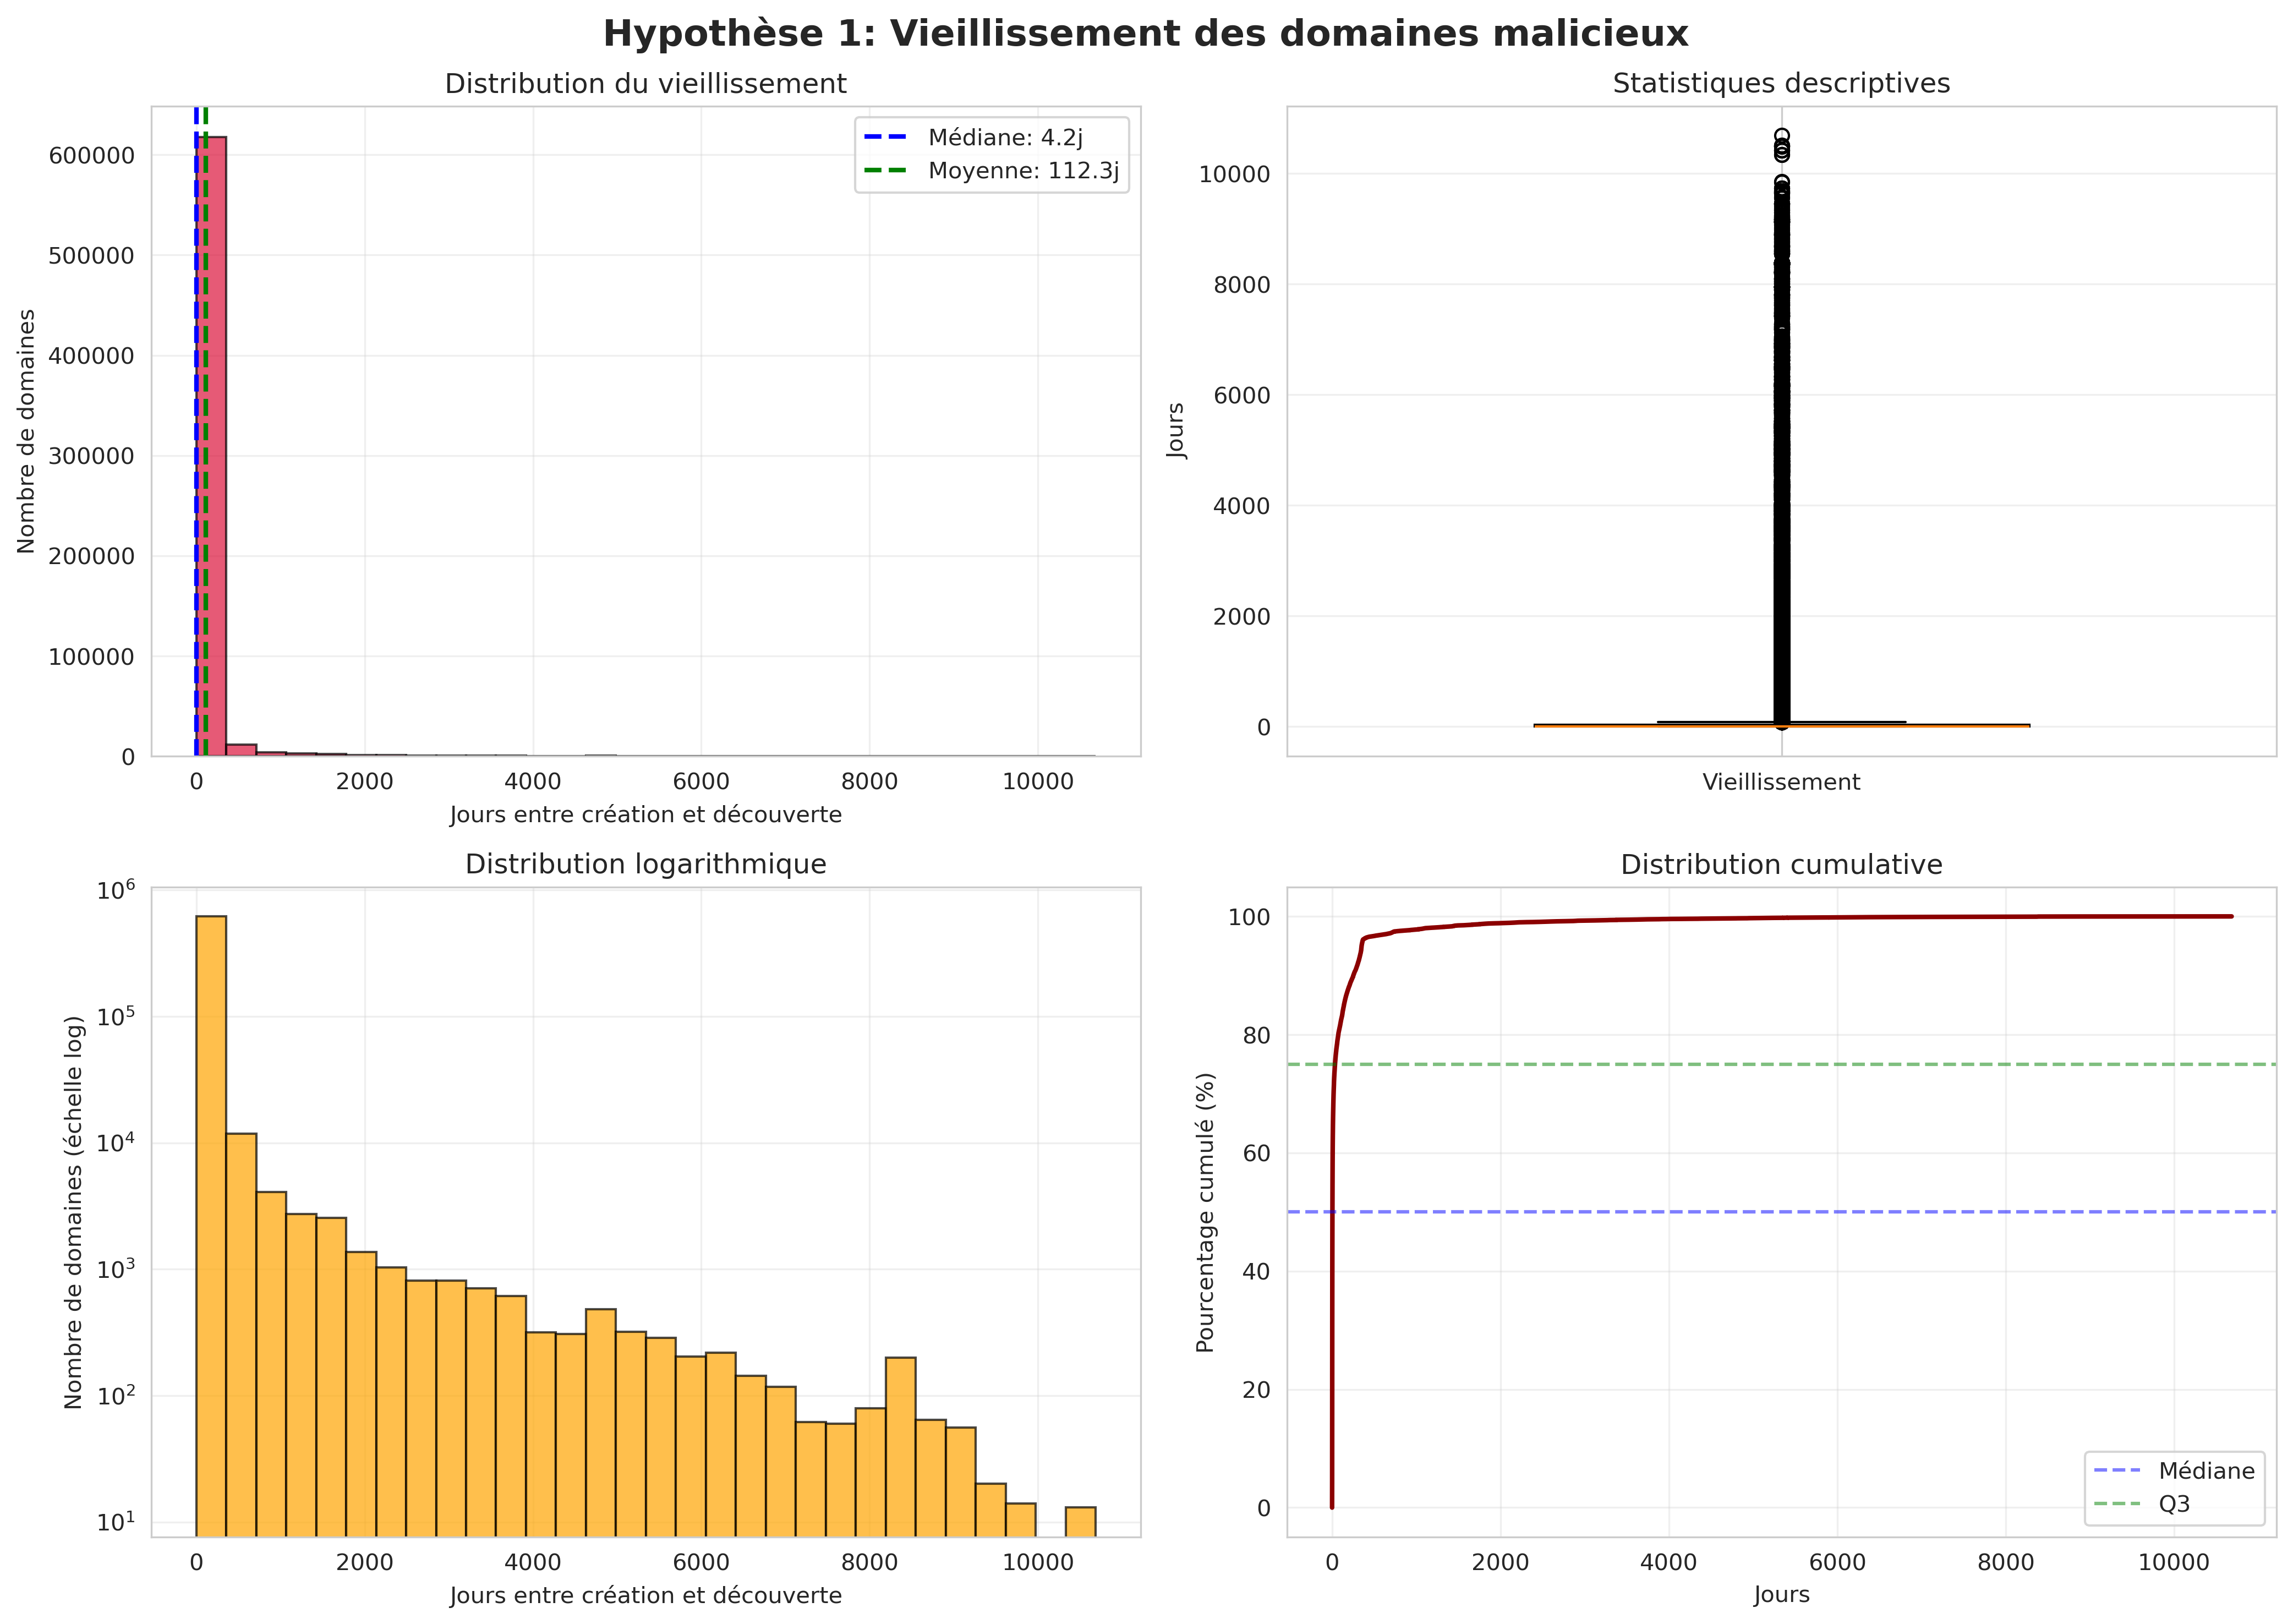
\includegraphics[width=\linewidth]{analysis_results/graphs_sample/hypothesis1_aging_full.png}
    \caption{hypothesis1\_aging\_full.png}
    \label{fig_app:analysis_results/graphs_sample/hypothesis1_aging_full.png}
\end{figure*}

\begin{figure*}[ht]
    \centering
    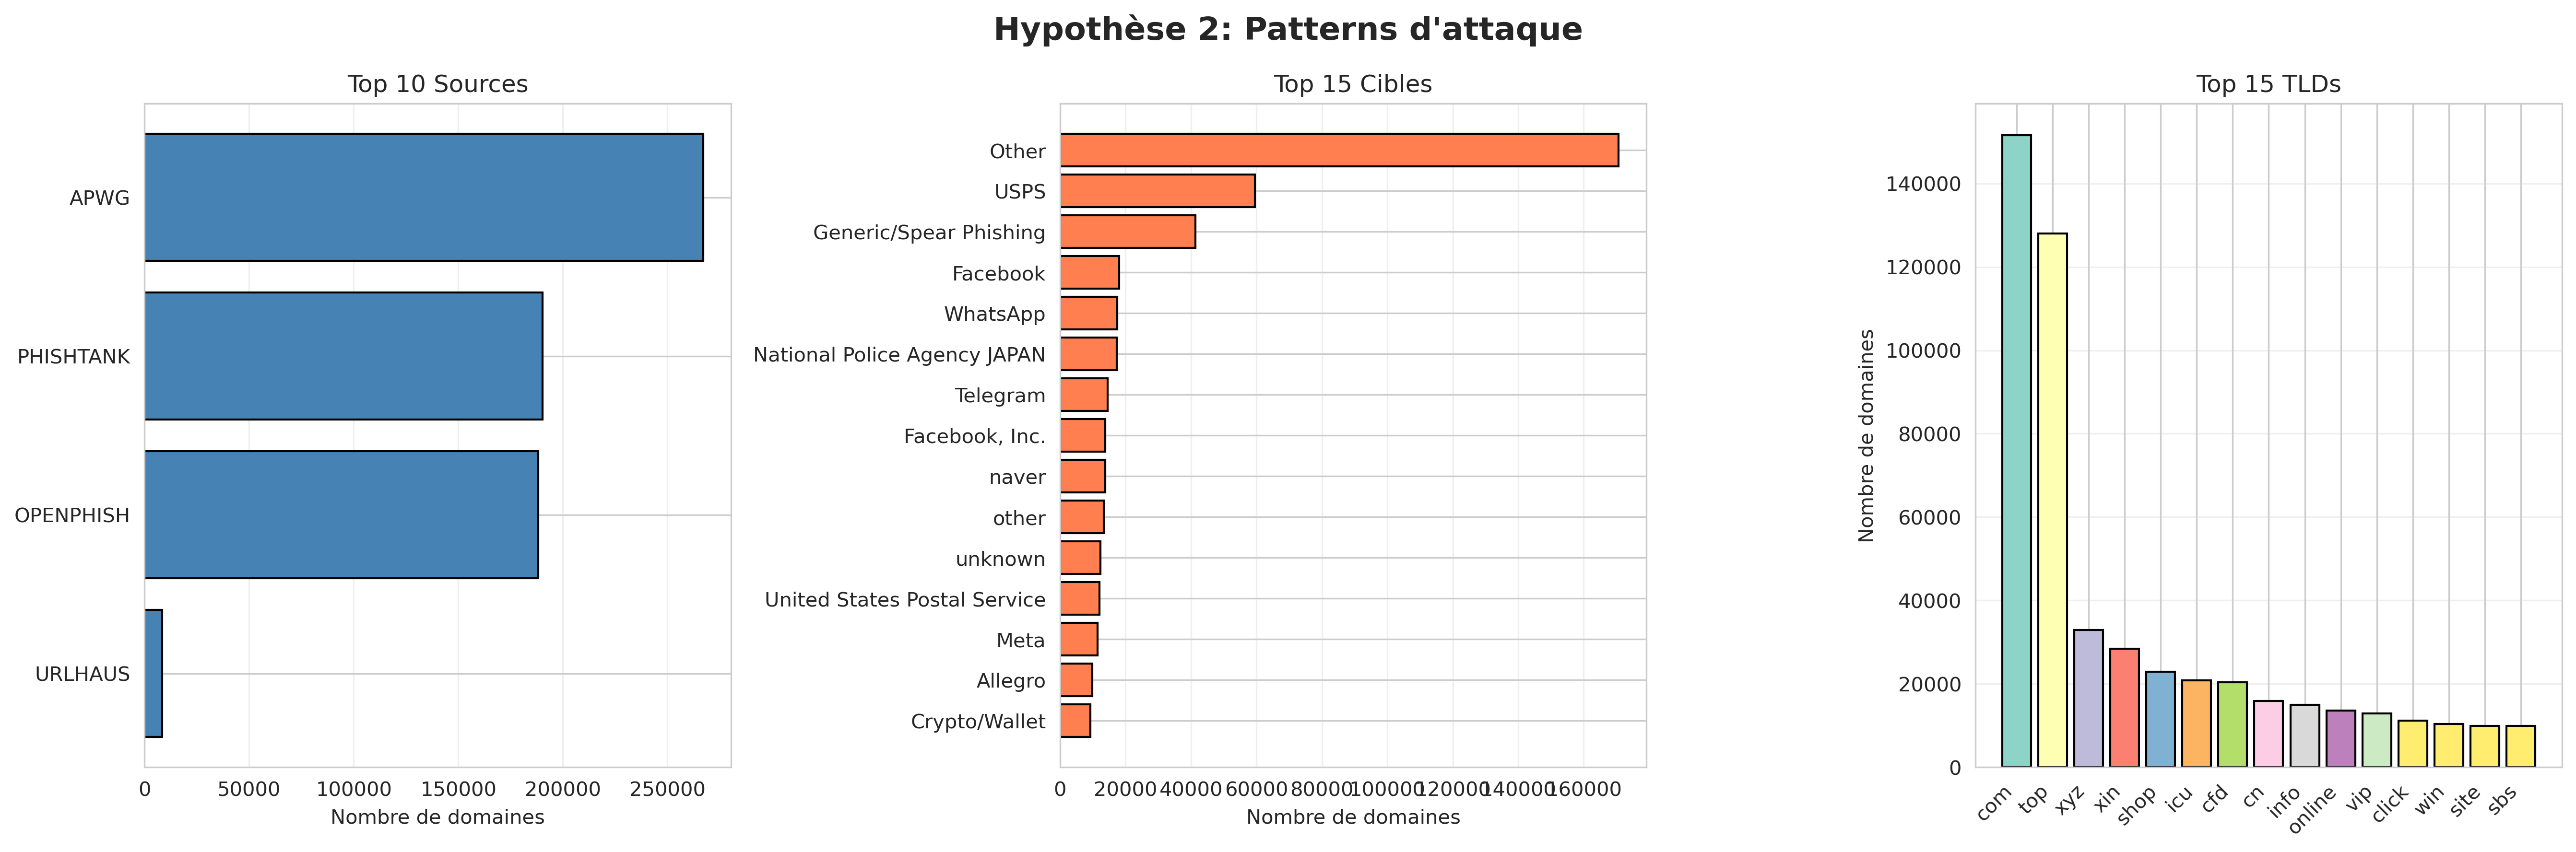
\includegraphics[width=\linewidth]{analysis_results/graphs_sample/hypothesis2_patterns_full.png}
    \caption{hypothesis2\_patterns\_full.png}
    \label{fig_app:analysis_results/graphs_sample/hypothesis2_patterns_full.png}
\end{figure*}

\begin{figure*}[ht]
    \centering
    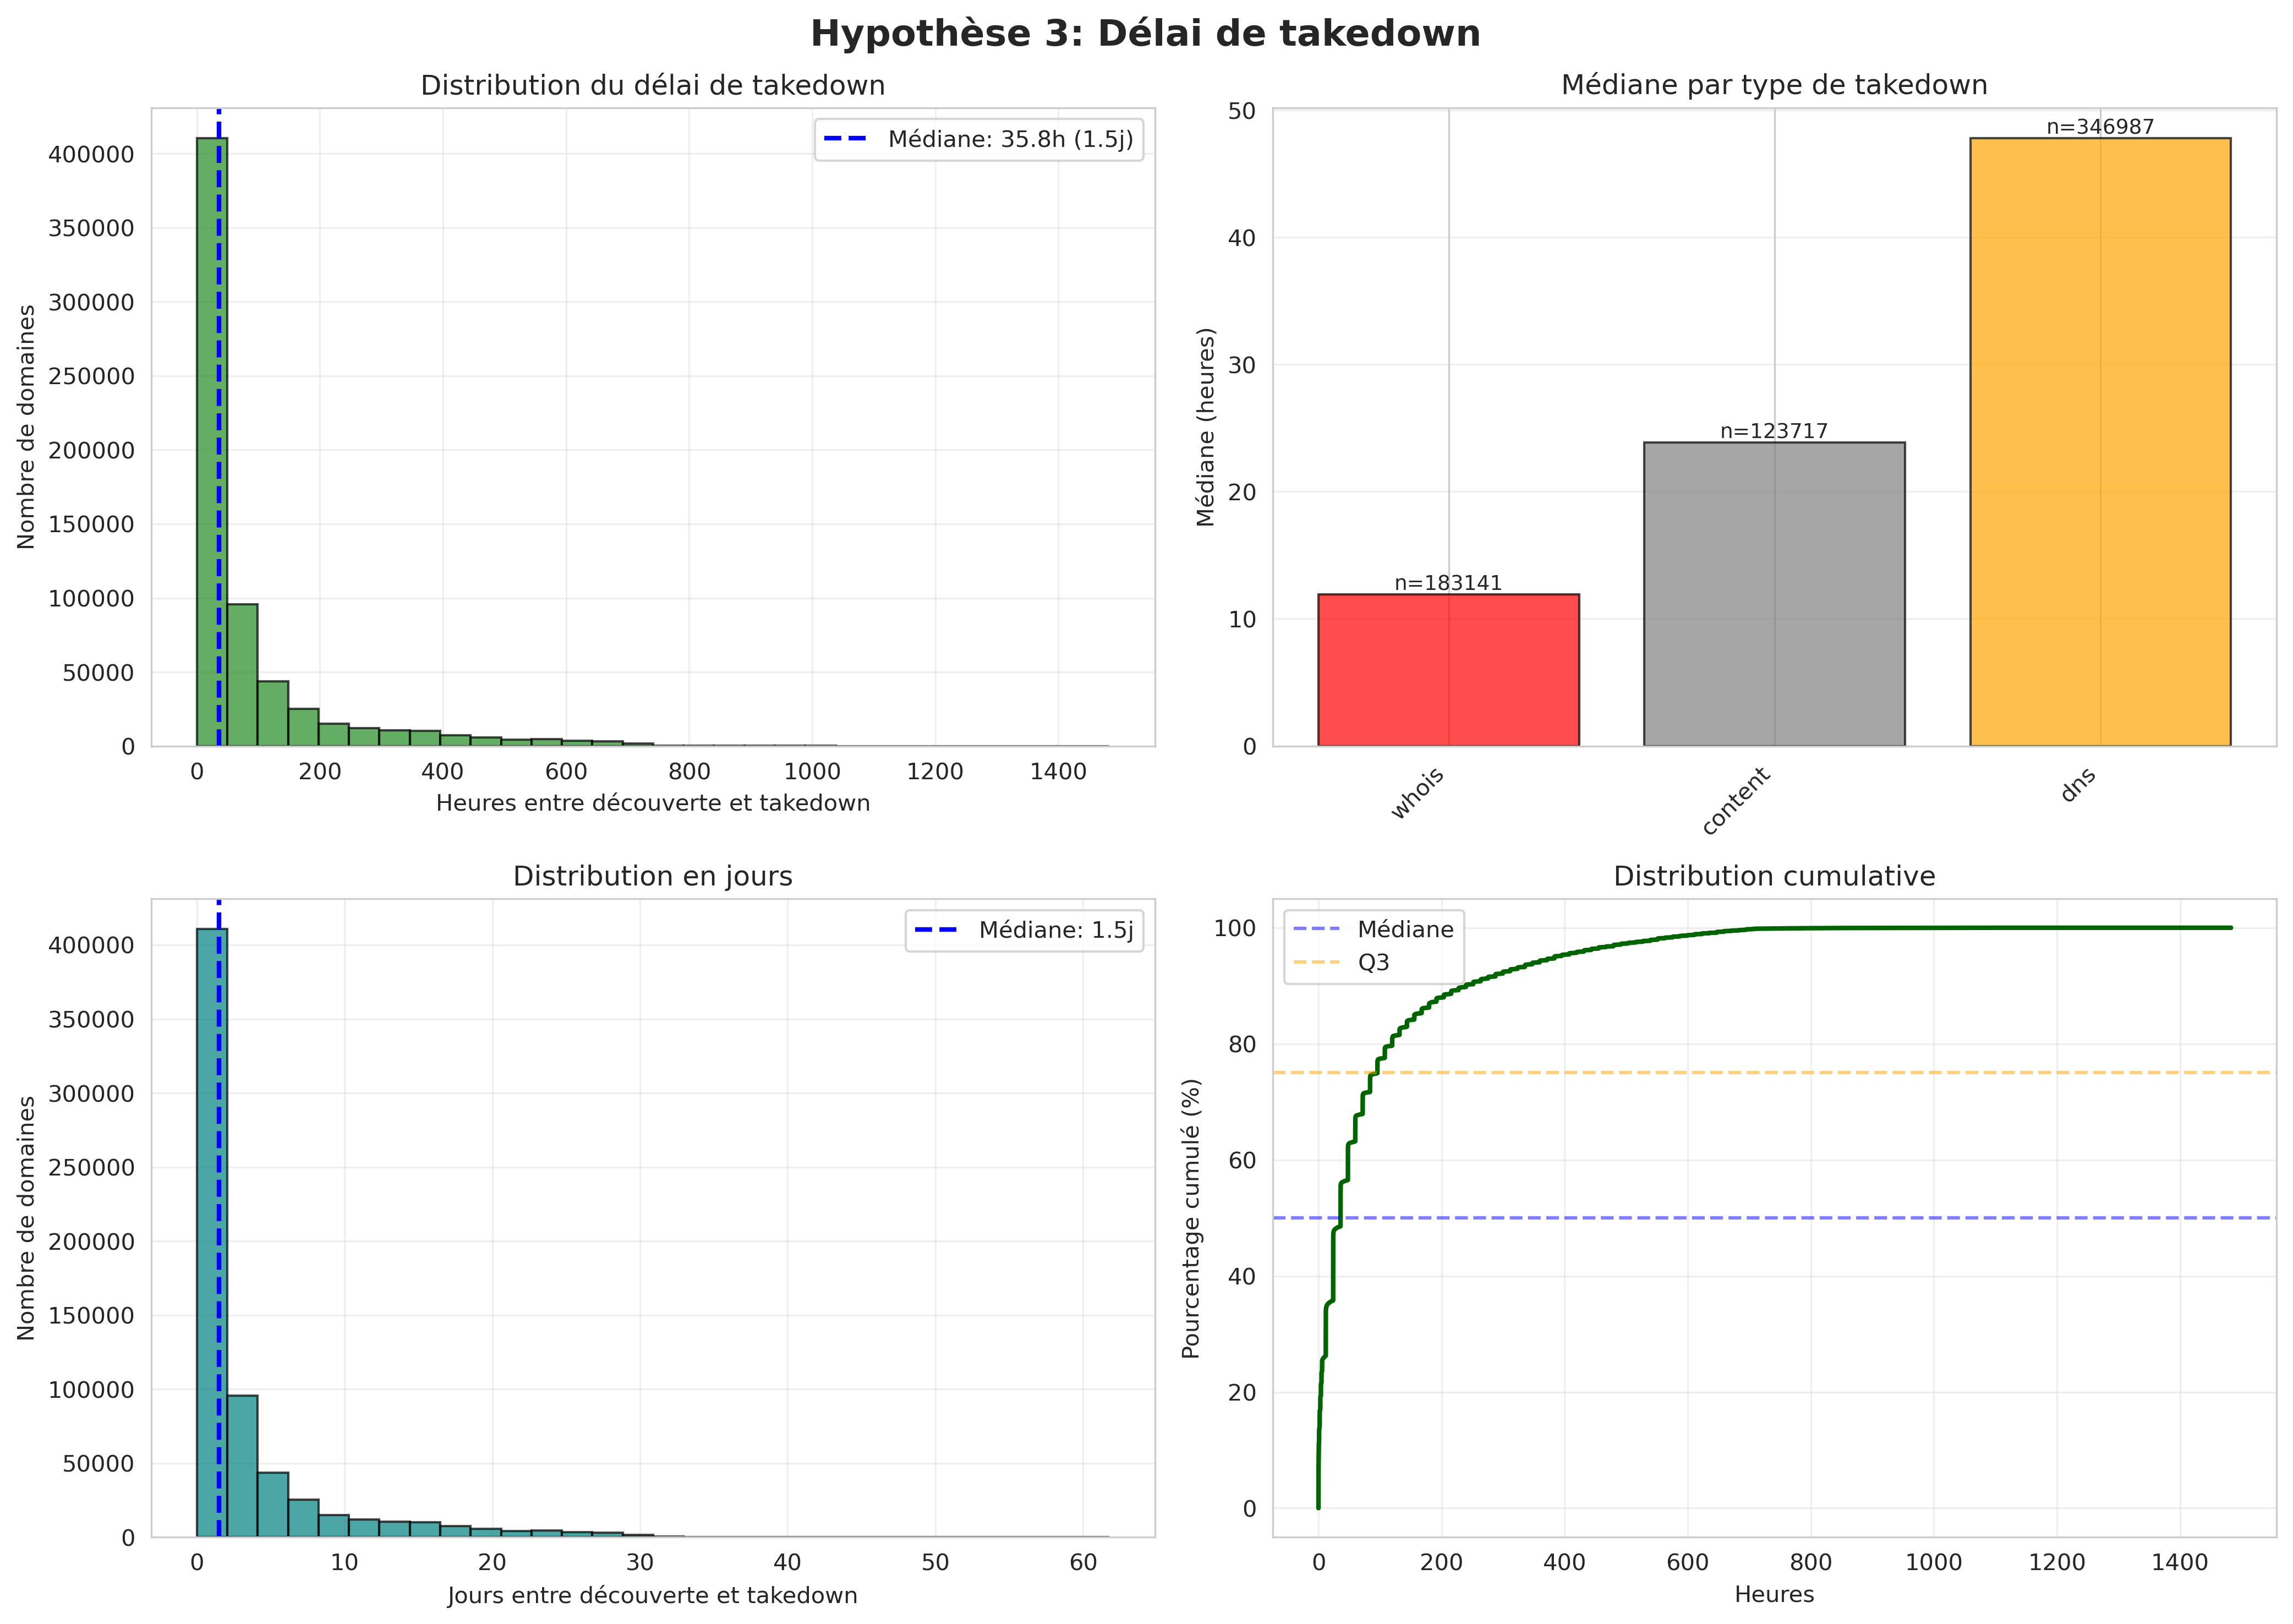
\includegraphics[width=\linewidth]{analysis_results/graphs_sample/hypothesis3_takedown_full.png}
    \caption{hypothesis3\_takedown\_full.png}
    \label{fig_app:analysis_results/graphs_sample/hypothesis3_takedown_full.png}
\end{figure*}

\begin{figure*}[ht]
    \centering
    
\includegraphics[width=\linewidth]{analysis_results/graphs_jpg/quarterly_attack_volume.jpg}
    \caption{quarterly\_attack\_volume.jpg}
    \label{fig_app:analysis_results/graphs_jpg/quarterly_attack_volume.jpg}
\end{figure*}

\begin{figure*}[ht]
    \centering
    
\includegraphics[width=\linewidth]{analysis_results/graphs_jpg/global_monthly_age_trend.jpg}
    \caption{global\_monthly\_age\_trend.jpg}
    \label{fig_app:analysis_results/graphs_jpg/global_monthly_age_trend.jpg}
\end{figure*}

\begin{figure*}[ht]
    \centering
    
\includegraphics[width=\linewidth]{analysis_results/graphs_jpg/dist_age_log.jpg}
    \caption{dist\_age\_log.jpg}
    \label{fig_app:analysis_results/graphs_jpg/dist_age_log.jpg}
\end{figure*}

\begin{figure*}[ht]
    \centering
    
\includegraphics[width=\linewidth]{analysis_results/graphs_jpg/annual_aging_strategies.jpg}
    \caption{annual\_aging\_strategies.jpg}
    \label{fig_app:analysis_results/graphs_jpg/annual_aging_strategies.jpg}
\end{figure*}

\begin{figure*}[ht]
    \centering
    
\includegraphics[width=\linewidth]{analysis_results/graphs_jpg/strategic_ratio_tld.jpg}
    \caption{strategic\_ratio\_tld.jpg}
    \label{fig_app:analysis_results/graphs_jpg/strategic_ratio_tld.jpg}
\end{figure*}

\begin{figure*}[ht]
    \centering
    
\includegraphics[width=\linewidth]{analysis_results/graphs_jpg/strategic_ratio_registrars.jpg}
    \caption{strategic\_ratio\_registrars.jpg}
    \label{fig_app:analysis_results/graphs_jpg/strategic_ratio_registrars.jpg}
\end{figure*}

\begin{figure*}[ht]
    \centering
    
\includegraphics[width=\linewidth]{analysis_results/graphs_jpg/aging_by_brand.jpg}
    \caption{aging\_by\_brand.jpg}
    \label{fig_app:analysis_results/graphs_jpg/aging_by_brand.jpg}
\end{figure*}

\begin{figure*}[ht]
    \centering
    
\includegraphics[width=\linewidth]{analysis_results/graphs_jpg/domain_length_vs_age.jpg}
    \caption{domain\_length\_vs\_age.jpg}
    \label{fig_app:analysis_results/graphs_jpg/domain_length_vs_age.jpg}
\end{figure*}

\begin{figure*}[ht]
    \centering
    
\includegraphics[width=\linewidth]{analysis_results/graphs_jpg/weekend_gap_analysis.jpg}
    \caption{weekend\_gap\_analysis.jpg}
    \label{fig_app:analysis_results/graphs_jpg/weekend_gap_analysis.jpg}
\end{figure*}

\begin{figure*}[ht]
    \centering
    
\includegraphics[width=\linewidth]{analysis_results/graphs_jpg/monthly_seasonality.jpg}
    \caption{monthly\_seasonality.jpg}
    \label{fig_app:analysis_results/graphs_jpg/monthly_seasonality.jpg}
\end{figure*}

\begin{figure*}[ht]
    \centering
    
\includegraphics[width=\linewidth]{analysis_results/graphs_jpg/whois_update_vs_age.jpg}
    \caption{whois\_update\_vs\_age.jpg}
    \label{fig_app:analysis_results/graphs_jpg/whois_update_vs_age.jpg}
\end{figure*}

\begin{figure*}[ht]
    \centering
    
\includegraphics[width=\linewidth]{analysis_results/graphs_jpg/late_weaponization_comparison.jpg}
    \caption{late\_weaponization\_comparison.jpg}
    \label{fig_app:analysis_results/graphs_jpg/late_weaponization_comparison.jpg}
\end{figure*}

\begin{figure*}[ht]
    \centering
    
\includegraphics[width=\linewidth]{analysis_results/graphs_jpg/survival_vs_age.jpg}
    \caption{survival\_vs\_age.jpg}
    \label{fig_app:analysis_results/graphs_jpg/survival_vs_age.jpg}
\end{figure*}

\begin{figure*}[ht]
    \centering
    
\includegraphics[width=\linewidth]{analysis_results/graphs_jpg/takedown_resistance_by_age.jpg}
    \caption{takedown\_resistance\_by\_age.jpg}
    \label{fig_app:analysis_results/graphs_jpg/takedown_resistance_by_age.jpg}
\end{figure*}

\begin{figure*}[ht]
    \centering
    
\includegraphics[width=\linewidth]{analysis_results/graphs_jpg/aging_by_registrar.jpg}
    \caption{aging\_by\_registrar.jpg}
    \label{fig_app:analysis_results/graphs_jpg/aging_by_registrar.jpg}
\end{figure*}

\end{document}
